\subsection{Prioritized-Timed Colored Petri Nets}\label{petrinet}

Next we introduce the particular model of prioritised-timed
coloured Petri net considered as the graphical formalism for the language BPELRF. 
 
We use prioritised-timed coloured Petri nets (PTCPNs), 
which are
a prioritised-timed extension of coloured Petri nets \cite{Jensen97}. PTCPNs 
are supported by CPN Tools \cite{CPNTools}, which is a toolbox
developed originally by the \emph{CPN group} at the University of Aarhus. The maintenance and extension of CPNTools are now in charge
of the group \emph{Architecture of Information Systems}, chaired by Wil van der Aalst, at Technische Universiteit Eindhoven.
Priorities were also introduced in Petri nets to extend the descriptive 
power of the model \cite{Bau96,BestK92,Pet81}, usually by
associating priority levels with transitions and modifying the firing
rule to prevent the firing of a transition when another one with
higher priority is enabled. Note that this feature is really useful  for describing some activities
in the language BPELRF.

In PTCPNs, places have an associated colour set (data types). 
Each token has then an attached data value
({\em token colour}),
which belongs to the colour to which the token is
associated. We will use timed colours, for which the first component
will be a non-negative integer value, representing the data value,
and the second component will be the token timestamp,
a natural number representing the time at which the 
token will be available.

There is also a discrete global clock that represents
the total time elapsed in the system model. Moreover, arcs have also 
an associated inscription ({\em arc expressions}),
constructed using variables, constants, operators
and functions. 
To evaluate an arc expression we need to
bind the variables that are part of the expression with their current value, that is, this binding
consists of assigning a value to the variables that appear in the
arc inscription. These values are then used to
select the token colours that must be removed or added when
firing the corresponding transition.

Arc expressions can also have associated time information
both for place-transition and transition-place arcs.
However, only time inscriptions are needed
in output arcs, and even, when all the output arcs
of a transition have the same time inscription,
there is a shorthand notation in CPN Tools
by which this time information is associated with
the transition instead of the output arcs.

The time inscription associated with a transition 
is used to specify the delay that must be added to the
current value of the global clock for
every token generated by the firing of the transition.

Transitions can also have associated guards, which
are Boolean expressions that can prevent their firing.
Thus, when a transition has a guard, it must evaluate to
true for the binding to be enabled,
otherwise the binding is disabled and 
the transition cannot be fired. 

\begin{definition} [(Prioritised-Timed Coloured Petri Nets)]
A prioritised-timed coloured Petri net is a tuple \ptcpntuple, where: %\footnote{
%We use the classical notation on Petri nets to denote the
%precondition and postcondition of both places and transitions:
%%
%\[ \forall x \in P\,\cup\,T\,:\,
%\precond{x} = \{ y \,|\, (y,x) \in A\}~~~~~
%   x^{\bullet} = \{ y \,|\, (x,y) \in A\}
%\]
%}:
%%
\begin{itemize}
\item $P$ is a finite set of {\em places}, with colours
in the set $\Sigma$. Thus, in our case, colours 
will be pairs $(n,x)\in \nnul \times \nnul$, where $n$ is
the token value and $x$ its timestamp.
%
\item $T$ is a finite set of {\em transitions} ($P\cap T = \emptyset$).
%
\item $A \subseteq (P\times T)\,\cup\,(T \times P)$ is a
set of directed {\em arcs}.
%
\item $\Sigma$ is a finite set of non-empty colour sets. These colour sets can be timed or untimed. For simplicity,
we only use non-negative integer variables and, therefore, the colour sets are: 
$\nnul \times \nnul$ for the timed version and $\nnul$ for the untimed version. Thus, in our case, colours 
will be pairs $(n,x)\in \nnul \times \nnul$ or just $n$, where $n$ is
the token value and $x$ its timestamp.
%
\item $V$ is a finite set of {\em typed variables} in $\Sigma$, 
i.e. ${\it Type}(v) \in \Sigma$, for all $v \in V$.
%
%
\item $G\,:\, T \longrightarrow {\it EXPR}_V$ is the
{\em guard function}, which assigns a Boolean
expression
to each transition, i.e. ${\it Type}(G(t))={\it Bool}$. 
%
\item $E\,:\, A \longrightarrow {\it EXPR}_V$ is the
{\em arc expression function}, which assigns an expression
to each arc, such that ${\it Type}(E(a)) = {\cal B}(\nnul)$,
which corresponds to untimed arcs, since, as mentioned above,
we only attach time delays to transitions.

\item $\lambda$ is the {\em labelling function}, defined
both on places and transitions.

\item $D\,:\,T \longrightarrow \nnul \times \nnul$, which
is the {\em delay function}, which associates a time
interval to each transition. For $D(t)=[d_1,d_2]$,
this means that a uniform probability function will
be used when $t$ is fired to select the specific discrete
delay in that time interval. This is a particularity of CPNTools \cite{CPNTools}.
%
\item $\pi\,:\,T \longrightarrow \nnul$ is the
{\em priority function}, which assigns a priority level
to each transition. In CPNTools, the lower value, the higher priority, that is, $0$ is the highest priority.
\end{itemize}

In this definition, ${\it EXPR}_V$ denotes the
expressions constructed using the variables in $V$,
with the same syntax admitted by CPN Tools. Notice again that we only use here non-negative integer variables for simplicity, but
our model can be easily extended to other variable types.
\end{definition}

\begin{definition} [(Markings)]
Given a PTCPN $N=\ptcpntuple$,
a marking $M$ is defined as a function
$M\,:\,P \longrightarrow {\cal B}(\Sigma)$,
which assigns a multiset of colours to each place
(which can be empty). 

A timed marking of a PTCPN $N$ is a pair $(M,x)$, where
$M$ is a marking of $N$ and $x$ is the current system time instant.
%
%
Initial markings are those markings for which
the timestamp of every token is $0$,
and all variable places are marked with a single
token $(0,0)$.
A marked prioritized-timed coloured Petri net (MPTCPN)
is then defined as a triple $(N,M,x)$, where
$N$ is a PTCPN, and $(M,x)$ a timed marking of it.
%
\end{definition}

We define the semantics for MPTCPNs in a similar way as in \cite{Jensen2009}, 
now taking into account that transitions have associated priorities.
We first introduce the notion of {\em binding}, then
the {\em enabling condition} and finally the {\em firing rule}
for MPTCPNs.

The variables of a transition $t$ are denoted $\mathit{Var(t)\subseteq V}$ and consist of the free variables
appearing in the guard of the transition and in the arc expressions connected to it.

\begin{definition} [(Bindings)]
Let $N=\ptcpntuple$ be a PTCPN.
A {\em binding} of a transition $t \in T$ is a function
$b$ that maps each variable $v \in {\it Var}(t)$
into a value $b(v) \in \Sigma$.
We will denote by $B(t)$ the set of all possible bindings
for the transition $t \in T$. 

Given an expression $e \in {\it EXPR}_V$, we will denote 
by $e\langle b \rangle$ the evaluation of $e$ for the
binding $b$.

A {\em binding element} is then defined as a pair
$(t,b)$, where $t \in T$ and $b \in B(t)$.
The set of all binding elements is denoted by $\mathit{BE}$.
\end{definition}

\begin{definition}[(Enabling condition)]\label{permitidas}
Let $N=\ptcpntuple$ be a PTCPN,
and $(M,x)$ a timed marking of it.
We say that a 
binding element $(t,b) \in \mathit{BE}$
is {\em enabled} at the time instant $x'$ in the timed marking
$(M,x)$ if and
only if the following conditions are fulfilled:

\begin{enumerate}
\item $x' \geq x$.
%
\item $G(t)\langle b \rangle = {\it true}$.
%
\item For all $p \in \precond{t}$,
$E(p,t)\langle b\rangle_{x'} \preceq M(p)$, 
where 
%
$E(p,t)\langle b \rangle_{x'}$ consists of the same
colours as $E(p,t)\langle b \rangle$, but 
replacing their timestamp (which was $0$) by $x'$.
%
%the notation $C_{+x}$ is used to represent the
%colour multiset obtained from $C$ by delaying its timestamps
%by $x$ time units:
%%
%\[
%C_{+x}(n,y) = \left\{
%\begin{array}{cl}
%C(n,y-x)~~ & {\rm if}\;y \geq  x\\
%0        & {\rm otherwise}
%\end{array}
%\right.
%\]
%
\item There is no other binding element $(t',b') \in {\it BE}$
fulfilling the previous conditions  such that $\pi(t') < \pi(t)$.
% INVERTIDAS LAS PRIORIDADES, PARA EVITAR PROBLEMAS,
% AHORA EL CERO ES LA MAXIMA PRIORIDAD.
%
%
\item $x'$ is the smallest time value for which there exists
a binding element $(t,b)$ fulfilling these conditions.
%
\end{enumerate}
%
\end{definition}

\begin{definition} [(Firing rule)]
Let $N=\ptcpntuple$ be a PTCPN,
$(M,x)$ a timed marking of $N$, and an enabled
binding element $(t,b) \in {\it BE}$ at 
instant $x'$ in the timed marking $(M,x)$.

The firing of $(t,b)$ at instant $x'$ is non-deterministic,
depending on the chosen delay $d \in \nnul$ for the transition.
This delay is randomly selected in the interval given by $D(t)$. 
%This delay is chosen according to a uniform probability distribution. 
Thus, the new timed marking $(M',x')$ is: 
%
\[
  \forall p \in P\,:\,
  M'(p) = M(p) \ominus E(p,t)\langle b \rangle_{x'} + E(t,p)\langle b
 \rangle_{d+x'}
\]
%
\end{definition}

\begin{figure}


\hspace*{1.0cm}
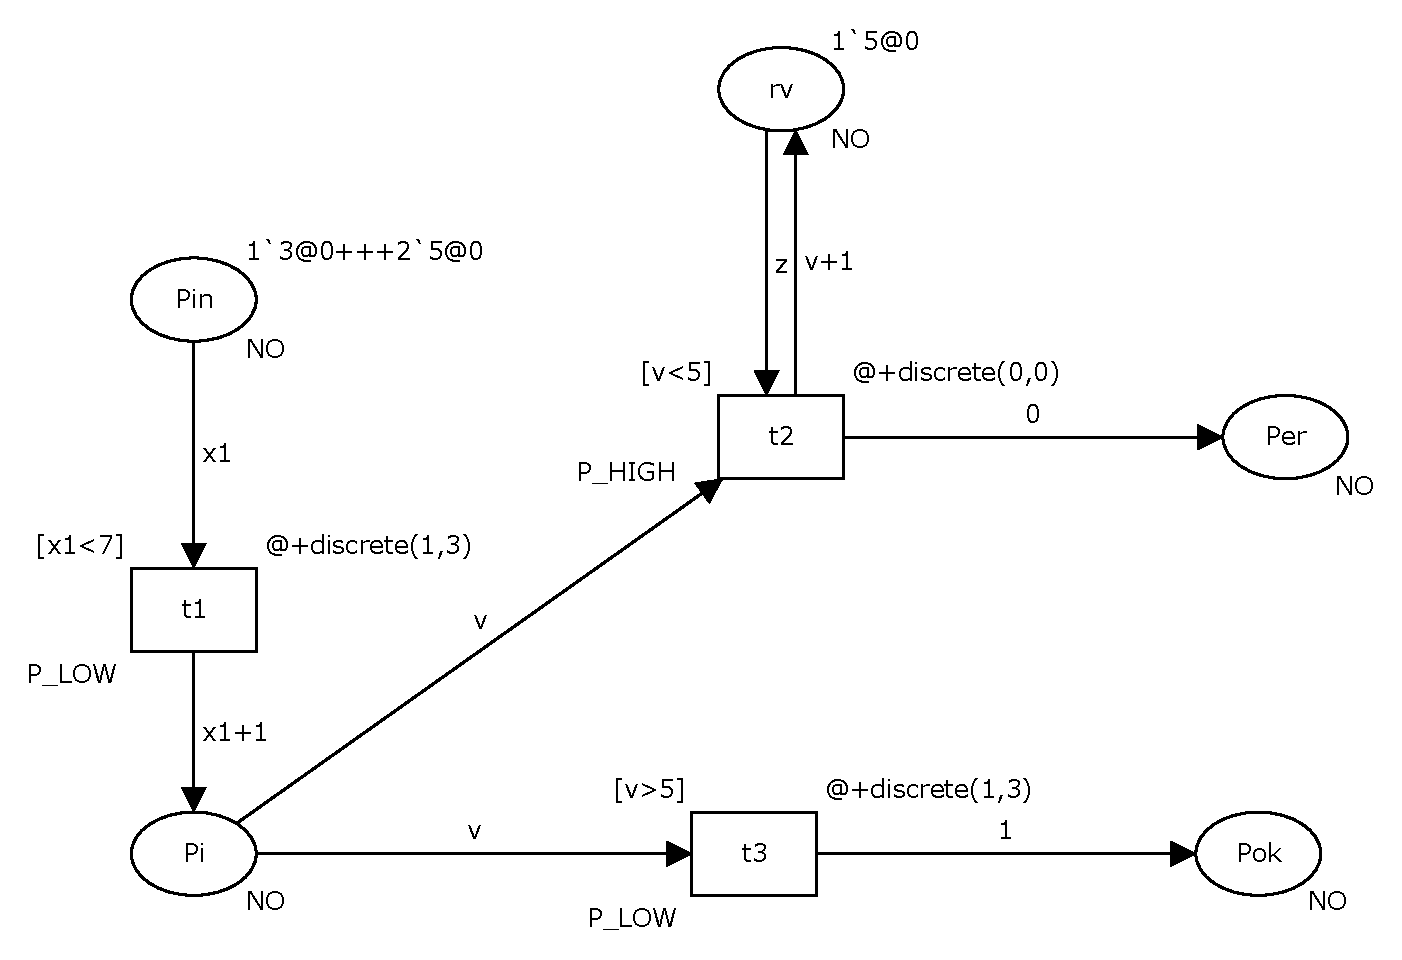
\includegraphics[width=11.5cm]{Figures/figure2_scp.eps}
% 
\caption{\label{red1}Graphical view of a PTCPN.}
\end{figure}

\begin{example} Let us consider the marked PTCPN depicted in Figure \ref{red1}, 
obtained from CPNTools examples. 
% 
Observe that timed colour tokens in CPN Tools are drawn
using the notation $n`v@x$,
meaning that we have $n$ instances of a timed colour token 
with colour value $v$ and {\em timestamp} $x$, which correspond to $n.(v,x)$
according to our formal notation. Besides, the symbol `+++'
is there used to represent the union of timed
multisets. 

Thus, $p_{\it in}$ is initially marked with one token
of colour $(3,0)$, and two tokens of colour $(5,0)$,
and the place ${\it rv}$ has one token with colour
$(5,0)$.  Transitions are labelled
with their associated guard, time interval and priority
information. 
Arcs are labelled with the corresponding expressions,
in which no time delays appear, as we are considering
that only transitions have associated time delays.

From the initial marking we can see that
only transition $t_1$ can be fired (at instant $0$), and
any token of those in $p_{\it in}$ can be used for
that purpose.  Taking $(5,0)$ we get the binding $x=5$,
which fulfils the transition guard.
The firing of $t_1$ with this binding removes
one instance of $(5,0)$ from $p_{\it in}$,
and produces a new token on $p_i$.
The timestamp of this new token is a discrete value
in the interval $[1,3]$ (let us say $3$).
Thus, considering the output
arc inscription we get a token $(6,3)$  on $p_i$.

Now, transition $t_1$ must fire again twice (until $p_{\it in}$ 
becomes empty), due to the time constraints of this model. 
As a result we may obtain in $p_i$ the following marking
$\{1.(4,3), 1.(6,1),$
$ 1.(6,3)\}$ (the timestamp values depend on the values
chosen from the interval $[1,3]$).
% 
The only transition that can be fired at this marking
is $t_3$, because due to the time constraints 
we must first use the token $(6,1)$
and $t_2$ cannot be fired using this token.
The firing of $t_3$ produces a new token on $p_{\it ok}$,
whose colour value must be $1$, and the timestamp
depends again on the chosen delay in the time interval
$[1,3]$. For instance, we could obtain the 
colour token $(1,4)$. 

Two tokens now remain in $p_i$, with colours  $(4,3)$ and 
$(6,3)$, and $t_2$ becomes the only transition
enabled (due to condition (4) of Def.\ \ref{permitidas}).
Its firing removes the token $(4,3)$ from $p_i$,
the token on the place ${\it rv}$ changes to $1.(5,3)$,  
and creates a new token on $p_{\it er}$, with colour $(0,3)$. 
%
% 
Finally, the remaining token $(6,3)$ on $p_i$ 
only allows us to fire $t_3$, generating a new token
on $p_{\it ok}$, with value $1$ and a timestamp
depending on the delay chosen for its firing.
\end{example}


%In \cite{Buc03} there is a model that
%extends Merlin's nets by including dynamic priorities and resources.
%
%The particular model that we use is also an extension of Merlin's
%nets, 
%% but it is simpler than that considered in \cite{Buc03}.
%including priorities and three transition types ({\em black,\,grey\,} and
%{\em white\,}). All transitions are assigned both a time interval
%and a static priority. The time interval restricts the instants at
%which a transition is allowed to be fired. {\em White}\, transitions
%are not forced to fire when their clock reaches its latest firing
%time, grey transitions must fire once their clock reaches that value, 
%and black  transitions
%must fire immediately, once they fulfil all the required conditions. 
%Of course, in the
%event of a conflict, any transition of those involved in the conflict 
%can be fired (whichever type it has), although we take into account 
%priorities to resolve the conflicts. Thus, priorities are only
%used in the case of conflict, when at a given marking two or more
%transitions are simultaneously enabled, then only those with 
%the maximum priority are allowed to be fired at that moment.
